% Appendices of report.tex: the learned models explained in detail, for teaching.
% Included after \appendix. Every number is the implementation's (src/apno) or a measured record.

\section{Neural networks from the ground up}
\label{app:basics}

\Cref{app:basics,app:fno,app:pinn,app:compare} explain the learned models of this study in enough
detail to rebuild them. This appendix covers the building blocks they share.
\Cref{app:fno} covers the Fourier neural operator and \cref{app:pinn} the physics-informed network,
each exactly as implemented in \texttt{src/apno/models}. \Cref{app:compare} sets the three models
side by side. Throughout, $\bm\theta$ denotes all the trainable parameters of a model.

\subsection{A network is a parameterised function}

The simplest network, and the one the PINN uses, is the \emph{multilayer perceptron} (MLP). It
maps an input vector $\bm x\in\mathbb R^{n_0}$ to an output $\bm y$ by alternating affine maps with
a fixed nonlinear function $\sigma$, applied element by element:
\begin{equation}
  \bm h^{0} = \bm x,\qquad
  \bm h^{\ell} = \sigma\!\bigl(\bm W^{\ell}\bm h^{\ell-1} + \bm b^{\ell}\bigr)\quad(\ell = 1,\dots,L),\qquad
  \bm y = \bm W^{L+1}\bm h^{L} + \bm b^{L+1}.
  \label{eq:mlp}
\end{equation}
\begin{itemize}
  \item The weight matrices $\bm W^\ell\in\mathbb R^{n_\ell\times n_{\ell-1}}$ and bias vectors
    $\bm b^\ell$ are the parameters, $n_\ell n_{\ell-1} + n_\ell$ of them per layer.
  \item $L$ is the \emph{depth}; $n_\ell$ is the \emph{width} of layer $\ell$.
  \item The PINN's network maps 3 inputs through $L = 7$ hidden layers of 96 units to one output.
    It has $(3\cdot96+96) + 6\,(96\cdot96+96) + (96+1) = 56{,}353$ parameters, plus the
    circulation $\Gamma$.
\end{itemize}

\paragraph{Why the nonlinearity matters.}
Without $\sigma$, \cref{eq:mlp} collapses to a single affine map, however deep it is. With a
nonlinear $\sigma$, a wide enough network can approximate any continuous function on a bounded set
to any accuracy (the universal approximation property). It says nothing about how hard the right
parameters are to \emph{find}, which is the whole difficulty in practice.

\paragraph{Activation functions.}
\Cref{fig:activations} compares the three activation functions relevant here.
\begin{itemize}
  \item \emph{tanh} is smooth and bounded, and has non-zero derivatives of every order.
  \item \emph{GELU}, $z\,\Phi(z)$ with $\Phi$ the standard normal distribution function, is a
    smooth version of the ReLU.
  \item \emph{ReLU}, $\max(z, 0)$, is piecewise linear: its second derivative is zero everywhere
    except at $z = 0$.
\end{itemize}
The choice matters for a PINN. A ReLU network is piecewise linear in its inputs, so every second
derivative of its output is zero almost everywhere, yet the full-potential residual is built from
second derivatives of the potential. This is why PINNs use tanh. The FNO only needs function values,
not derivatives, so it uses GELU.

\paragraph{Initialisation.}
Training starts from random parameters. PyTorch draws each affine layer's weights and biases
uniformly from $(-1/\sqrt{n_{\ell-1}},\ 1/\sqrt{n_{\ell-1}})$, which keeps each layer's initial
outputs of moderate size whatever its width. Fixing the random seed makes a run repeatable.

\begin{figure}[t]
\centering
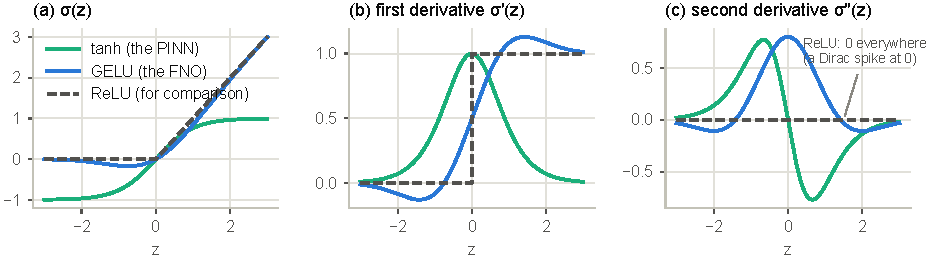
\includegraphics[width=\textwidth]{activations.pdf}
\caption{The activation functions used here and their derivatives. A PINN's loss contains
derivatives of the network with respect to its \emph{inputs}, so the activation's own derivatives
appear in the equations being solved. A ReLU network's second derivatives are zero almost
everywhere.}
\label{fig:activations}
\end{figure}

\subsection{Training is optimisation}

\paragraph{The loss.}
A \emph{loss} $\mathcal L(\bm\theta)$ is a single number that measures how wrong the network is.
\begin{itemize}
  \item In \emph{supervised} learning, as for the FNO, it compares the network's output with known
    answers: here, SU2's fields for the training cases.
  \item In \emph{physics-informed} learning, as for the PINN, there are no answers. The loss is how
    badly the network's output violates the governing equations and boundary conditions.
\end{itemize}
Training means finding parameters that make the loss small.

\paragraph{Gradient descent.}
The basic method steps against the gradient,
\begin{equation}
  \bm\theta \leftarrow \bm\theta - \eta\,\nabla_{\bm\theta}\mathcal L,
\end{equation}
with a \emph{learning rate} $\eta$.

\paragraph{Stochastic gradients.}
Computing the loss over all the data at every step is expensive, so the gradient is estimated
from a small random subset:
\begin{itemize}
  \item the FNO uses a \emph{mini-batch} of 8 cases per step, and one pass over all the training
    cases is an \emph{epoch};
  \item the PINN uses one set of 20,000 random collocation points, redrawn every 1,000 steps.
\end{itemize}
The noise in such estimates is tolerated, and it can even help an optimiser leave poor regions.

\subsection{Automatic differentiation}
\label{app:autodiff}

\paragraph{Reverse mode.}
Gradients are never derived by hand. PyTorch records every elementary operation of the forward
computation as a graph and then applies the chain rule backwards through it (\emph{reverse-mode
automatic differentiation}, or backpropagation). The gradient of a scalar loss with respect to all
parameters then costs a small multiple of one forward pass, however many parameters there are.

\paragraph{Derivatives with respect to the inputs.}
A PINN needs a second kind of derivative: of the network's \emph{output} with respect to its
\emph{inputs}, such as $\partial\psi/\partial\xi$. These come from the same machinery. In the code,
\begin{center}
\cmd{torch.autograd.grad(f.sum(), xi, create\_graph=True)}
\end{center}
returns $\partial f/\partial\xi$ at every collocation point at once. Summing first is legitimate
because each point's output depends only on that point's input, so the derivative of the sum with
respect to the $n$-th input is the derivative of the $n$-th output.

\paragraph{Differentiating a derivative.}
The flag \cmd{create\_graph=True} records the derivative computation itself as part of the graph,
so the derivative can be differentiated again. This nesting is what PINNs are built from:
\begin{itemize}
  \item the potential PINN differentiates $\psi$ once for the velocity;
  \item it differentiates again for the divergence in the residual;
  \item training then differentiates the loss with respect to $\bm\theta$ through both levels.
\end{itemize}
\Cref{app:pinnderivs} counts what that costs.

\subsection{Optimisers}

\paragraph{Adam.}
Adam~\cite{kingma2015adam} keeps running averages of the gradient $\bm g_t$ and of its element-wise
square, corrects their start-up bias, and scales each parameter's step by its own gradient history:
\begin{equation}
  \bm m_t = \beta_1\bm m_{t-1} + (1-\beta_1)\bm g_t,\quad
  \bm v_t = \beta_2\bm v_{t-1} + (1-\beta_2)\bm g_t^2,\quad
  \bm\theta_t = \bm\theta_{t-1} - \eta_t\,\frac{\bm m_t/(1-\beta_1^t)}{\sqrt{\bm v_t/(1-\beta_2^t)} + \epsilon},
  \label{eq:adam}
\end{equation}
with $\beta_1 = 0.9$, $\beta_2 = 0.999$ and $\epsilon = 10^{-8}$. Because every parameter gets its
own step size, Adam copes with losses whose sensitivity varies by orders of magnitude between
parameters. That is common in both networks here.

\paragraph{AdamW.}
AdamW~\cite{loshchilov2019adamw}, used for the FNO, adds \emph{decoupled} weight decay: it also
shrinks every weight by $\eta_t\lambda\bm\theta$ at each step ($\lambda = 10^{-4}$). This is
separate from the gradient, which discourages large weights without distorting Adam's scaling.

\paragraph{Learning-rate schedules.}
Large steps make fast early progress; small steps settle into a minimum. Both networks lower
$\eta_t$ as training proceeds:
\begin{equation}
  \text{FNO (cosine): }\ \eta_e = \tfrac12\eta_0\bigl(1 + \cos(\pi e/E)\bigr),\qquad
  \text{PINN (exponential): }\ \eta_k = \eta_0\,(\eta_1/\eta_0)^{k/K}.
\end{equation}
Here $e$ is the epoch of $E$ (300 in the final runs), $k$ the step of $K = 30{,}000$, and
$\eta_0 = 10^{-3}$, $\eta_1 = 10^{-4}$.

\paragraph{L-BFGS.}
L-BFGS~\cite{liu1989lbfgs} is a quasi-Newton method, used to finish the PINN's training. It builds
an approximation of the inverse Hessian from the last $m = 50$ pairs
\begin{equation}
  \bm s_k = \bm\theta_{k+1} - \bm\theta_k,\qquad \bm y_k = \nabla\mathcal L_{k+1} - \nabla\mathcal L_k,
\end{equation}
turns the gradient into a Newton-like search direction, and chooses the step length by a line
search satisfying the strong Wolfe conditions. Near a minimum it converges far faster than Adam.
It needs two things Adam does not:
\begin{itemize}
  \item \emph{A fixed objective.} If the collocation points changed between iterations, $\bm y_k$
    would mix a change in the function with a change in its sampling, and the line search would
    chase a moving target.
  \item \emph{Accurate arithmetic.} $\bm y_k$ is a difference of two nearly equal gradients, so in
    float32, with about 7 significant digits, it soon becomes mostly round-off. L-BFGS therefore
    runs in float64, on the CPU, because the Apple GPU has no float64.
\end{itemize}

\subsection{Generalisation, and what it means for each model}

A supervised model is judged on cases it never saw. The data are therefore split three ways:
\begin{itemize}
  \item a \emph{training set}, used to fit $\bm\theta$;
  \item a \emph{validation set}, used to choose hyperparameters and when to stop;
  \item a \emph{test set}, used once, for the final score.
\end{itemize}
\emph{Early stopping} keeps the parameters from the epoch with the lowest validation loss, and stops
when it has not improved for a set number of epochs (the \emph{patience}). Training several
\emph{seeds} (initialisations and batch orders) shows how much of a result is luck.

A PINN has no training set and nothing to generalise to: it fits one case. Its only test is the
comparison with SU2, which it never sees. The lesson of this study is that for a PINN a small loss
is not the same as a right answer (\cref{app:lessons}).

\subsection*{Questions}
\begin{enumerate}[label=Q\arabic*., leftmargin=*]
\item \textit{Why could a ReLU network not serve as the PINN here?}\newline
The full-potential residual contains second derivatives of the potential. A ReLU network is
piecewise linear, so its second derivatives vanish almost everywhere, and the residual would not
see the curvature that the equation constrains.
\item \textit{Why does the L-BFGS phase keep one fixed set of collocation points?}\newline
Its curvature pairs and its line search assume one deterministic function. Resampled points would
make every gradient difference partly sampling noise.
\item \textit{What does early stopping select, and from which data?}\newline
The epoch with the lowest validation loss. Test cases are never used for any choice.
\end{enumerate}

%---------------------------------------------------------------------------------------------------
\section{The Fourier neural operator in detail}
\label{app:fno}

\subsection{Learning an operator}

An ordinary network maps vectors to vectors. A \emph{neural operator} maps functions to functions.
Here the input function is the geometry and free stream, given as six fields over the grid, and the
output function is the flow state over the same grid:
\begin{equation}
\begin{aligned}
  \mathcal G:\quad \bm a(i,j) &= \bigl(\text{position},\ \text{ring index},\ \Ma,\ \cos\alpha,\ \sin\alpha\bigr)\\
  \longmapsto\quad \bm y(i,j) &= \text{the four targets of \cref{eq:targets}}.
\end{aligned}
\end{equation}
The operator is learned from 881 examples of the pair $(\bm a,\bm y)$. Ideally its parameters do
not depend on the grid, so a model trained at one resolution can be evaluated at another; the
measured resolution transfer error tests how far that holds here.

\subsection{From kernel integrals to Fourier multipliers}

A neural-operator layer replaces the matrix of an MLP by an integral operator acting on the hidden
function $\bm h(\bm z)$:
\begin{equation}
  \bm h_{\ell+1}(\bm z) = \sigma\!\left(\bm W\bm h_\ell(\bm z) + \int\kappa_{\bm\vartheta}(\bm z - \bm z')\,\bm h_\ell(\bm z')\,\mathrm d\bm z'\right).
\end{equation}
If the kernel $\kappa$ depends only on $\bm z - \bm z'$, the integral is a convolution. The
convolution theorem then turns it into a product in Fourier space,
\begin{equation}
  (\kappa * \bm h)(\bm z) = \mathcal F^{-1}\bigl[\hat\kappa(\bm k)\,\hat{\bm h}(\bm k)\bigr](\bm z).
\end{equation}
The FNO~\cite{li2021fno} learns $\hat\kappa$ directly: one complex $w\times w$ matrix
$\bm R_{\bm k}$ for each retained wavenumber $\bm k$, where $w$ is the number of hidden channels.
High wavenumbers are dropped. On a grid, $\mathcal F$ is the fast Fourier transform, so the layer
costs $O(N\log N)$ for $N$ nodes, and it couples every node to every other in a single layer.

\subsection{The Fourier layer as implemented}

The hidden state is a tensor $\bm h\in\mathbb R^{B\times w\times N_I\times(N_J+P)}$: batch,
channels, nodes around the airfoil, and nodes outward including the padding. One Fourier layer
(\cref{fig:fnoarch}, bottom) does five things.
\begin{enumerate}
  \item \emph{Transform}: $\hat{\bm h} = \mathrm{rfft2}(\bm h)$. This is a full FFT along $i$ and a
    real FFT along $j$, which keeps only the non-negative $j$-frequencies, since the negative ones
    are their complex conjugates.
  \item \emph{Truncate and mix}: keep $i$-frequencies $k_i\in\{0,\dots,23\}\cup\{-24,\dots,-1\}$
    and $j$-frequencies $k_j\in\{0,\dots,7\}$. At each kept mode, mix the channels with that mode's
    own complex matrix,
    \begin{equation}
      \hat o_{b,o,\bm k} = \sum_{c=1}^{w}\hat h_{b,c,\bm k}\,R_{c,o,\bm k},
    \end{equation}
    and set every other mode to zero. Positive and negative $k_i$ need separate weight tensors
    (\cmd{w\_pos} and \cmd{w\_neg}), because the real FFT halves only the $j$ axis.
  \item \emph{Inverse transform} back to the grid.
  \item \emph{Pointwise path}: add $\bm W\bm h + \bm b$, a $1\times1$ convolution, which mixes
    channels at each node with no spatial coupling.
  \item \emph{Activation}: apply GELU, except after the last layer.
\end{enumerate}

\paragraph{Why the pointwise path is needed.}
The spectral path can carry only $48\times8$ modes. The pointwise path passes everything else, the
fine detail that nonlinearities create in particular, and it is not tied to periodicity at all.
Without it, every layer's output would be a smooth, band-limited field.

\begin{figure}[t]
\centering
\begin{tikzpicture}[
  font=\scriptsize,
  blk/.style={draw=black!55, rounded corners=2pt, fill=black!3, align=center, inner sep=3pt,
              minimum height=11mm, text width=17mm},
  fl/.style={blk, fill=blue!7},
  arr/.style={-{Stealth[length=1.8mm]}, black!65, semithick},
  shp/.style={font=\tiny, text=black!60, align=center}]
\node[blk] (a) {input $\bm a$\\6 channels};
\node[blk, right=4mm of a] (P) {lift $P$\\$1\times1$ conv\\$6\to48$};
\node[blk, right=4mm of P] (pad) {zero-pad\\$P(N_J)$ rows\\in $j$};
\node[fl, right=4mm of pad] (F) {Fourier layer\\$\times\,4$};
\node[blk, right=4mm of F] (crop) {crop the\\padding};
\node[blk, right=4mm of crop] (Q) {project $Q$\\$48\to128\to4$};
\node[blk, right=4mm of Q] (y) {output $\bm y$\\4 channels};
\foreach \u/\v in {a/P, P/pad, pad/F, F/crop, crop/Q, Q/y} \draw[arr] (\u) -- (\v);
\node[shp, below=1mm of a] {$8\times6\times128\times49$};
\node[shp, below=1mm of P] {$8\times48\times128\times49$};
\node[shp, below=1mm of pad] {$8\times48\times128\times57$};
\node[shp, below=1mm of F] {$8\times48\times128\times57$};
\node[shp, below=1mm of crop] {$8\times48\times128\times49$};
\node[shp, below=1mm of Q] {$8\times4\times128\times49$};
% the Fourier layer, expanded
\begin{scope}[yshift=-30mm]
\node[blk, text width=12mm] (h) {$\bm h$};
\node[blk, right=5mm of h, text width=15mm] (fft) {rfft2\\over $(i,j)$};
\node[fl, right=5mm of fft, text width=30mm] (R) {keep $|k_i|<24$, $k_j<8$;\\multiply each mode by\\its own $48\times48$ complex $\bm R_{\bm k}$};
\node[blk, right=5mm of R, text width=15mm] (ifft) {inverse\\rfft2};
\node[circle, draw=black!55, right=5mm of ifft, inner sep=1pt] (plus) {$+$};
\node[blk, right=5mm of plus, text width=12mm] (act) {GELU\\$\sigma$};
\node[blk, below=5mm of R, text width=40mm, minimum height=8mm] (W) {pointwise $\bm W\bm h + \bm b$ ($1\times1$ conv)};
\node[blk, right=5mm of act, text width=10mm] (h2) {$\bm h'$};
\draw[arr] (h) -- (fft); \draw[arr] (fft) -- (R); \draw[arr] (R) -- (ifft); \draw[arr] (ifft) -- (plus);
\draw[arr] (plus) -- (act); \draw[arr] (act) -- (h2);
\draw[arr] (h.south) |- (W.west); \draw[arr] (W.east) -| (plus.south);
\node[shp, above=0.5mm of fft] {$\hat{\bm h}$: $8\times48\times128\times29$, complex};
\end{scope}
\node[font=\scriptsize\bfseries, black!70, anchor=south west] at ([yshift=7mm]h.north west) {one Fourier layer, expanded};
\end{tikzpicture}
\caption{The FNO as implemented, with tensor shapes (batch, channels, $i$, $j$) for a batch of 8 at
the $128\times49$ training resolution, with the selected width of 48. The projection is two
$1\times1$ convolutions with a GELU between them. At $256\times97$ the same
weights see $8\times48\times256\times113$ after padding, and the same $48\times8$ retained modes.
Bottom: one Fourier layer.}
\label{fig:fnoarch}
\end{figure}

\paragraph{Where the parameters are.}
\Cref{tab:fnoparams} counts the parameters. Almost all of them, 99.8\,\%, are spectral weights.
The model has about $7.1$ million real parameters, and the training set holds
$881\times4\times128\times49 = 22.1$ million target values. Weight decay, early stopping and
the truncation itself are what keep it from memorising them.

\begin{table}[t]
\centering\small
\caption{Parameters of the selected FNO (width 48, modes $24\times8$, 4 layers). A complex weight
counts as two real numbers.}
\label{tab:fnoparams}
\begin{tabular}{@{}lll r@{}}
\toprule
Part & Shape & Per part & Real numbers\\
\midrule
Lift $P$ & $48\times6$ weights $+\,48$ biases & & 336\\
Spectral weights $\bm R$, 4 layers & $2\times(48\times48\times24\times8)$ complex per layer & 1,769,472 & 7,077,888\\
Pointwise $\bm W$, 4 layers & $48\times48 + 48$ per layer & 2,352 & 9,408\\
Projection $Q$ & $(48\times128+128) + (128\times4+4)$ & & 6,788\\
\midrule
Total & & & 7,094,420\\
\bottomrule
\end{tabular}
\end{table}

\subsection{Working in the O-grid's index space}

\paragraph{Index space, not physical space.}
The FFT treats the grid as a uniform rectangle of nodes. The physical grid is curved and strongly
stretched: its first wall spacing is $2\times10^{-3}$ chords, while near the outer boundary the
spacing is chord-sized. A convolution in index space is translation-invariant in $(i,j)$, not in
$(x,y)$, so the geometry reaches the model only through the position channels. The model has to
learn what an index-space pattern means at each physical location.

\paragraph{Around the airfoil, periodicity is exact.}
Node $i = N_I$ is node $i = 0$, so the FFT along $i$ involves no approximation. Mode $k_i$ is
$k_i$ cycles per circuit of the airfoil at any $N_I$. This is what lets the same $\bm R_{\bm k}$
mean the same thing at $128$ and at $256$ nodes.

\paragraph{Outward, the field is not periodic.}
A plain FFT along $j$ would wrap the outer boundary onto the wall. Zero-padding by $P$ rows puts a
buffer between them:
\begin{equation}
  P = \tfrac{1}{6}(N_J - 1):\qquad
  \frac{48 + 8}{48} = \frac{96 + 16}{96} = \frac{7}{6},
\end{equation}
so the padded column spans the same $\eta$ at both resolutions. The discrete period in $\eta$ is
$(N_J + P)\,\Delta\eta = (N_J + P)/(N_J - 1)$, and it differs slightly: 57/48 against 113/96.
From 1 to 26 October the rule was $P = \mathrm{round}\bigl(\tfrac{3}{16}(N_J - 1)\bigr) - 1$ (8 and
17 rows), which makes the period $19/16$ at both, so that a learned radial mode means the same
physical frequency. On the trained networks 16 rows transferred better than 17, and the rule was
changed back (\cref{sec:fno}). The padded rows are zero only on entry. The layers write into them,
and they are cropped once, before the projection.

\paragraph{The transfer is still only first-order.}
At the end of the padding the field jumps back to the wall row's values, and that jump aliases
differently at the two resolutions. The measured transfer error is therefore not zero: on the
validation cases, the selected model's prediction at $128\times49$ differs from its prediction at
$256\times97$ by a relative L2 of 0.021 (0.035 with 17 rows). In the test scores this is the
factor of 1.7 between the two grids on in-range subcritical cases (\cref{tab:results}); with 17
rows it was 4.

\subsection{Inputs and outputs}

\paragraph{Inputs.}
The six input channels are given in \cref{sec:models}. The position channels are
$(x - \tfrac12,\ y)\,\ln(1+r)/r$. This keeps the direction of each node from mid-chord and
compresses its distance logarithmically: the outer circle at $r = 100$ maps to radius
$\ln101\approx4.6$, while the section is barely distorted. Without the compression, the far field
would dominate the coordinate values and the near-body detail would occupy a sliver of their range.

\paragraph{Outputs.}
The targets (\cref{eq:targets}) are each standardised per channel, over all training cases and
nodes: $z = (y - \mu_c)/s_c$. The network predicts $z$. A prediction is mapped back by inverting
the standardisation and then \cref{eq:targets}:
\begin{equation}
  \hat u = y_1 + \cos\alpha,\quad \hat v = y_2 + \sin\alpha,\quad
  \hat p = 1 + \tfrac12\gamma\Ma^2 y_3,\quad \hat\rho = 1 + \tfrac12\Ma^2 y_4.
\end{equation}

\subsection{Training}

\Cref{alg:fno} is the training loop as run. At $n = 896$ the training set is the 881 converged
cases among the first 896 Sobol points. An epoch is 111 mini-batches of 8, so 300 epochs are
33,300 AdamW steps, which took 36 minutes on the Apple GPU.

\Cref{fig:learning} shows the validation loss for each training-set size. Every curve still
improves at epoch 300: the best epochs are 274--297. The noise on each curve is the mini-batch
noise, filtered by the decaying learning rate. More data lowers the whole curve, but by less at
each doubling (\cref{tab:efficiency}).

\begin{algorithm}[t]
\caption{FNO training (\texttt{apno.models.train\_fno.train})}
\label{alg:fno}
\small
\begin{algorithmic}[1]
\Require training cases (the first $n$ Sobol points that converged), validation cases, seed
\State fit the per-channel standardiser on the training targets
\State $\bm X,\bm Z\gets$ features and standardised targets at every second node ($128\times49$)
\State initialise $\bm\theta$ from the seed; $v^\ast\gets\infty$
\For{epoch $e = 0,\dots,E-1$}
  \For{each mini-batch $b$ of 8 cases, in a fresh random order}
    \State $\mathcal L\gets\mathcal L_A$ (or $\mathcal L_B$) of $\mathrm{FNO}_{\bm\theta}(\bm X_b)$ against $\bm Z_b$
    \State $\bm\theta\gets\mathrm{AdamW}(\bm\theta,\nabla_{\bm\theta}\mathcal L)$
  \EndFor
  \State lower the learning rate (cosine); $v\gets$ validation loss
  \If{$v < v^\ast$} \State save $\bm\theta$ as the checkpoint; $v^\ast\gets v$; $e^\ast\gets e$
  \ElsIf{$e - e^\ast\ge30$} \State \textbf{stop}
  \EndIf
\EndFor
\State \Return the checkpoint (the epoch of lowest validation loss)
\end{algorithmic}
\end{algorithm}

\begin{figure}[t]
\centering
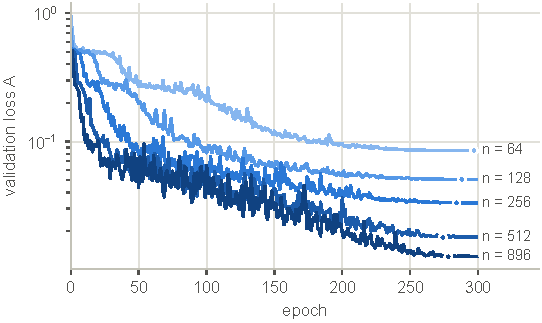
\includegraphics[width=0.66\textwidth]{learning_curves.pdf}
\caption{FNO validation loss per epoch for each training-set size $n$ (seed 0, loss A), darker
for larger $n$. Dots mark the epoch each run kept.}
\label{fig:learning}
\end{figure}

\subsection{What truncation does to a shock}

A truncated Fourier series of a function with a jump overshoots near the jump and oscillates on
both sides: the Gibbs phenomenon, an overshoot of about 9\,\% of the jump that does not shrink as
modes are added. \Cref{fig:truncation} applies the FNO's mode budget directly to the wall pressure
of the strongest showcase shock: the 24 lowest $i$-modes of each sign, out of 64, on the 128-node
training wall. The shock becomes a ramp with ripples on both sides.

The FNO is not a single filter. The pointwise paths and the nonlinearities generate the higher
frequencies that a filter alone would discard, so its own shocks are sharper than
\cref{fig:truncation}(a). The bias remains visible in the scores, though: its in-range shock
overshoot has median 0.42, against the floor's 0.19 (\cref{tab:shocks}).

\begin{figure}[t]
\centering
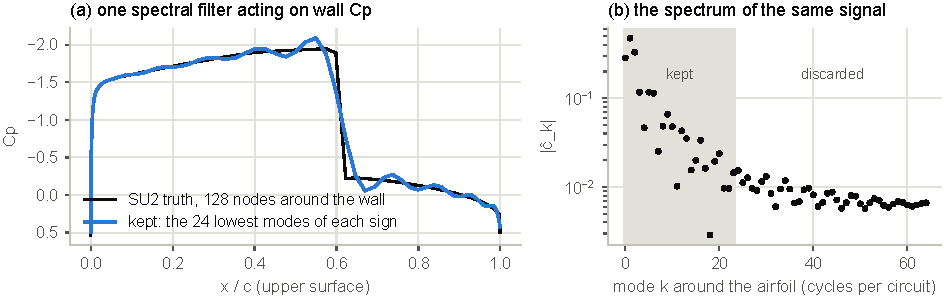
\includegraphics[width=\textwidth]{spectral_truncation.pdf}
\caption{(a) Wall $\Cp$ on the upper surface of \texttt{test\_in-0040} (SU2 truth at the
$128\times49$ training resolution), and the same signal keeping only the FNO's 24 lowest
$i$-modes of each sign. (b) The signal's Fourier amplitudes around the full wall. A shock puts
energy into every mode, and a slowly decaying tail is what a jump looks like in a spectrum.}
\label{fig:truncation}
\end{figure}

\subsection{Evaluation, and keeping the test set out}

\paragraph{Prediction.}
A prediction computes the six features on the case's own $256\times97$ grid, runs the network,
and inverts the target mapping. It takes 0.054\,s per case, about $4000$ times faster than an SU2
run.

\paragraph{Leakage guard.}
The data loader refuses to read a test split. Test inputs are read through a separate function that
returns only coordinates and free-stream values, never fields. A test case therefore cannot enter
training, normalisation or model selection by accident.

\subsection*{Questions}
\begin{enumerate}[label=Q\arabic*., leftmargin=*]
\item \textit{Why does a learned mode along $i$ mean the same thing at 128 and 256 nodes, while the $j$
direction needed a padding rule?}\newline
Along $i$ the grid is periodic with a period of one circuit at any $N_I$. Along $j$ the field is
not periodic, so it is padded; the period is then set by the $N_J + P$ padded samples and depends
on the choice of $P$. Matching the period exactly turned out to transfer worse on the trained
networks than matching the padded span.
\item \textit{How many complex weights does one Fourier layer hold, and why two tensors?}\newline
$2\times48\times48\times24\times8 = 884{,}736$. The real FFT halves only the $j$ axis, so positive
and negative $i$-frequencies are distinct modes, each with its own weights.
\item \textit{What was loss B meant to fix, and what happened?}\newline
Forces depend only on wall pressure, while a field loss is dominated by the many off-wall nodes.
Loss B adds the wall row with weight 10. In practice it was worse almost everywhere, and stopped
early at epoch 81 (\cref{sec:results}).
\item \textit{Why is the FNO's in-range subcritical error 1.7 times smaller on its training grid?}\newline
The resolution transfer is only first-order, because of the padding wrap; the same weights see
differently aliased fields at $256\times97$.
\end{enumerate}

%---------------------------------------------------------------------------------------------------
\section{The physics-informed neural network in detail}
\label{app:pinn}

\subsection{The idea}

A PINN~\cite{raissi2019pinn} represents the solution of \emph{one} problem as a network: a function
of continuous coordinates. It is trained so that the governing equations and boundary conditions
hold at many sampled points.
\begin{itemize}
  \item There is no training data. The equations supply the supervision, so the method can in
    principle solve a case nobody has solved.
  \item Derivatives are exact, by automatic differentiation, and there is no mesh to generate.
  \item The answer can be evaluated anywhere, at any resolution.
\end{itemize}
The price is that every new case is a fresh, non-convex optimisation, and its loss is a residual,
not an error.

\subsection{The network and its inputs}

The network is the MLP of \cref{eq:mlp} with 7 hidden layers of 96 tanh units. Its three inputs are
$(\cos2\pi\xi,\ \sin2\pi\xi,\ \eta)$, not $(x,y)$ and not $(\xi,\eta)$. Because $\xi$ enters only
through $\cos2\pi\xi$ and $\sin2\pi\xi$, the output satisfies $\psi(\xi + 1,\eta) = \psi(\xi,\eta)$
exactly: periodicity around the airfoil is built in, not learned. The full-potential network
outputs one scalar $\psi$ and has one more parameter, $\Gamma$, for 56,354 in all. The Euler network
outputs three, $(\ln\hat\rho,\ \hat u - \cos\alpha,\ \hat v - \sin\alpha)$, and has 56,547.

\paragraph{Why the circulation needs its own parameter.}
Around a lifting airfoil the potential is multivalued: one circuit around the body adds $\Gamma$ to
$\phi$. A network of $(\cos2\pi\xi, \sin2\pi\xi, \eta)$ is single-valued and cannot represent that
jump. The term $\Gamma\Theta_v$ carries it instead: $\Theta_v$ jumps by exactly one across the wake
cut, and its gradient, the velocity, is continuous there. The network therefore represents only
the single-valued remainder.

\subsection{Hard and soft constraints}

Every condition the solution must meet is either built into the representation (\emph{hard}),
holding for any $\bm\theta$, or added to the loss (\emph{soft}), holding only as well as the
optimiser manages. \Cref{tab:constraints} lists both formulations.

Each hard constraint removes a way to fail. Each soft one is something the optimiser may trade
against the others. The Euler PINN's failure here is this distinction at work: its far field was
soft, and the optimiser traded it away for fluid at rest. The full-potential PINN makes the far
field hard and puts the wall in the loss instead. A soft far field is not fatal in itself, though:
Wassing, Langer and Bekemeyer~\cite{wassing2025} keep it soft, weight the residual
$2\times10^4$ times more heavily, and succeed.

\begin{table}[t]
\centering\small
\caption{How each condition enters the two PINN formulations.}
\label{tab:constraints}
\begin{tabularx}{\textwidth}{@{}>{\raggedright\arraybackslash}p{0.2\textwidth}>{\raggedright\arraybackslash}X>{\raggedright\arraybackslash}X@{}}
\toprule
Condition & Euler PINN & Full-potential PINN\\
\midrule
Periodic around the airfoil & hard: inputs $\cos2\pi\xi$, $\sin2\pi\xi$ & hard: the same\\
Far field & soft: $(\hat\rho-1)^2 + |\hat{\vu} - \hat{\vu}_\infty|^2$ on 1,000 outer points, weight 10 & hard: $\psi(1-\eta) = 0$ on $\eta = 1$\\
Wall tangency & hard: normal component removed with weight $(1-\eta)^4$ & soft: $(\vu\cdot\hat{\bm n}_w)^2$ at 512 wall points, weight 10\\
Positive density & hard: $\hat\rho = \exp(\cdot)$ & hard: Bernoulli, base floored at $10^{-6}$\\
Constant total enthalpy & hard: pressure from $H_\infty$ & hard: Bernoulli at $H_\infty$\\
Irrotational, isentropic & not imposed & hard: $\vu = \nabla\phi$, $\hat p = \hat\rho^{\,\gamma}$\\
Momentum & residual (two equations) & identity\\
Continuity & residual & residual (the only equation)\\
Kutta condition & soft: $|\vu|^2 = 0$ at the trailing edge, weight 10 & soft: equal speeds at $\xi = \delta, 1-\delta$, weight 10\\
Circulation & implied by the velocity field & explicit parameter $\Gamma$\\
\bottomrule
\end{tabularx}
\end{table}

\subsection{Derivatives through the grid map}
\label{app:pinnderivs}

\paragraph{The chain rule through the map.}
The network is a function of $(\xi,\eta)$, but the equations are written in $(x,y)$. The map
\cref{eq:ogrid} links them, and its derivatives (the \emph{metric terms}) come from automatic
differentiation of the same function the mesh generator uses. By the chain rule,
\begin{equation}
  \begin{pmatrix}\phi_x\\ \phi_y\end{pmatrix}
  = \frac1J\begin{pmatrix} y_\eta & -y_\xi\\ -x_\eta & x_\xi\end{pmatrix}
    \begin{pmatrix}\phi_\xi\\ \phi_\eta\end{pmatrix},\qquad J = x_\xi y_\eta - x_\eta y_\xi .
\end{equation}

\paragraph{The divergence.}
The divergence of the mass flux $(f,g) = \rho(u,v)$ uses the strong conservation form
\cref{eq:strongform}. It is the same quantity, rearranged so that the metric terms sit inside the
derivatives, as in a finite-volume scheme. The test suite checks that uniform flow gives zero to
round-off through this operator on the curved grid.

\paragraph{The trailing edge.}
At the trailing-edge wall point $J = 0$, because $x_\xi = y_\xi = 0$ there. The velocity there is
$0/0$, and the code reports the Kutta stagnation value, zero, at that single point.

\paragraph{The cost of the derivatives.}
For one training step of the full-potential PINN, the derivatives nest as follows:
\begin{enumerate}
  \item a forward pass gives $\psi$ and hence $\phi$ at 20,000 points;
  \item a first differentiation gives $\phi_\xi$ and $\phi_\eta$, hence $u$, $v$, $\rho$ and
    $(f,g)$;
  \item a second differentiation, of $y_\eta f - x_\eta g$ with respect to $\xi$ and of
    $-y_\xi f + x_\xi g$ with respect to $\eta$, gives the residual $\mathcal R$, which involves
    second derivatives of $\psi$;
  \item backpropagation of the loss to $\bm\theta$ differentiates that whole graph once more.
\end{enumerate}
In effect the step computes third-order derivatives of the network. The Euler PINN's residual
needs only first derivatives of its outputs, because its fluxes are algebraic in the state. That is
why one full-potential Adam step cost 0.88\,s on the CPU against the Euler PINN's 0.60\,s, and
0.19\,s on the Apple GPU. \Cref{fig:pinngraph} draws the computation.

\begin{figure}[t]
\centering
\begin{tikzpicture}[
  font=\scriptsize,
  blk/.style={draw=black!55, rounded corners=2pt, fill=black!3, align=center, inner sep=3pt,
              minimum height=9mm, text width=24mm},
  net/.style={blk, fill=green!8},
  ad/.style={blk, fill=blue!6},
  arr/.style={-{Stealth[length=1.8mm]}, black!65, semithick}]
\node[blk] (pts) at (0,0) {collocation points\\$(\xi_n,\eta_n)$, $n\le20{,}000$};
\node[net, text width=28mm] (feat) at (0,-1.7) {features\\$(\cos2\pi\xi,\ \sin2\pi\xi,\ \eta)$};
\node[net] (mlp) at (0,-3.4) {MLP $7\times96$ tanh\\$\to\psi(\xi,\eta;\bm\theta)$};
\node[blk, text width=30mm] (map) at (4.1,0) {O-grid map $\bm x(\xi,\eta)$\\metrics $x_\xi, x_\eta, y_\xi, y_\eta, J$};
\node[blk, text width=30mm] (phi) at (4.1,-1.7) {$\phi = x\cos\alpha + y\sin\alpha$\\$+\ \Gamma\,\Theta_v(x,y) + \psi\,(1-\eta)$};
\node[ad, text width=30mm] (vel) at (4.1,-3.4) {differentiate once:\\$\phi_\xi,\phi_\eta\ \to\ u, v$ (metrics)};
\node[blk, text width=30mm] (loss) at (8.6,0) {$\mathcal L = \overline{\mathcal R^2} + 10\,\overline{(\vu\cdot\hat{\bm n}_w)^2}$\\$+\ 10\,(|\vu|^2_\delta - |\vu|^2_{1-\delta})^2$};
\node[ad] (res) at (8.6,-1.7) {differentiate again:\\strong-form $\mathcal R$};
\node[blk] (rho) at (8.6,-3.4) {Bernoulli $\hat\rho(|\vu|^2)$\\flux $\rho\vu$};
\node[ad, text width=21mm] (bp) at (12.4,0) {backpropagate:\\$\nabla_{\bm\theta,\Gamma}\mathcal L$};
\node[blk, text width=21mm] (opt) at (12.4,-1.7) {Adam step\\(then L-BFGS)};
\draw[arr] (pts) -- (feat); \draw[arr] (feat) -- (mlp); \draw[arr] (pts) -- (map);
\draw[arr] (map) -- (phi); \draw[arr] (mlp.east) -- (phi.south west); \draw[arr] (phi) -- (vel);
\draw[arr] (vel) -- (rho); \draw[arr] (rho) -- (res); \draw[arr] (res) -- (loss);
\draw[arr] (vel.north east) -- node[sloped, above, font=\tiny, black!65] {wall and Kutta points} (loss.south west);
\draw[arr] (loss) -- (bp); \draw[arr] (bp) -- (opt);
\draw[arr, dashed] (opt.south) |- ([yshift=-6mm]mlp.south) node[pos=0.75, below, font=\tiny, black!65] {update $\bm\theta,\Gamma$} -- (mlp.south);
\end{tikzpicture}
\caption{One training step of the full-potential PINN. Green: the network. Blue: automatic
differentiation. The residual needs two nested derivatives of the network with respect to its
inputs, and the update differentiates through both.}
\label{fig:pinngraph}
\end{figure}

\subsection{Collocation points}

\paragraph{Where the points fall.}
Each draw is 20,000 points uniform in $(\xi,\eta)$, which the map turns into points strongly
clustered at the body (\cref{fig:collocation}). In the first draw of the production run on
\texttt{test\_in-0022}, 11,018 points lie within 2.5 chords of mid-chord, a disk that is 0.06\,\%
of the domain's area. Two consequences follow:
\begin{itemize}
  \item A mean over these points weights each physical region by $1/J$. That favours the near field
    where the answer matters, but it also means the loss barely sees most of the domain.
  \item Points are redrawn every 1,000 Adam steps, so the network cannot satisfy the equation only
    at a fixed set of points and be wrong between them.
\end{itemize}

\paragraph{The trailing-edge exclusion.}
After each draw, the points within 0.02 chord of the trailing edge are dropped (225 in the draw
shown). The corner flow is singular there, and those few points would otherwise dominate the
loss.

\paragraph{Wall points.}
The 512 wall points sit at $\xi = (k + \tfrac12)/512$, half a spacing off the grid, so that none
falls on the degenerate trailing-edge point.

\begin{figure}[t]
\centering
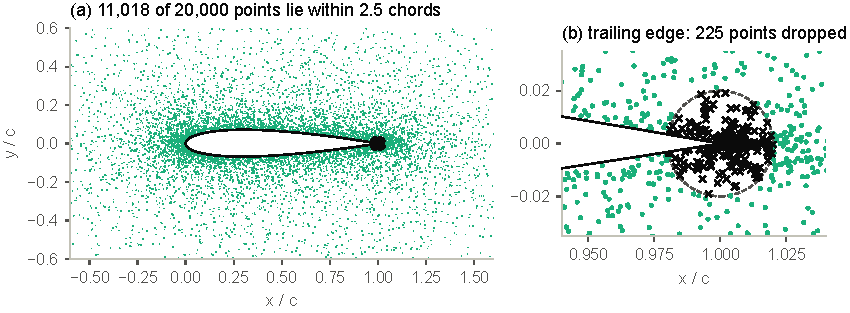
\includegraphics[width=\textwidth]{collocation.pdf}
\caption{The first draw of collocation points of the \texttt{pure} run on \texttt{test\_in-0022}
(seed 0, as drawn in production). Points uniform in $(\xi,\eta)$ crowd the section and its wake
line. Crosses: points inside the 0.02-chord trailing-edge exclusion (dashed circle), which are
dropped from the residual.}
\label{fig:collocation}
\end{figure}

\subsection{The loss and its weights}

\paragraph{One trade-off for several conditions.}
The loss \cref{eq:pinnloss} adds terms with different units and very different sizes and
sensitivities. Minimising a weighted sum finds one point on a trade-off between them. Only if the
network could satisfy every term exactly at once would the weights not matter, and with finite
networks and a singular corner it cannot. With fixed weights of 10, the \texttt{pure} runs ended
with residual $1$--$24\times10^{-3}$, wall term $0.5$--$21\times10^{-4}$ and Kutta term below
$6\times10^{-6}$ (\cref{tab:pinnruns}).

\paragraph{Gradient-norm balancing.}
Gradient-norm balancing~\cite{wang2021gradient} sets each weight from how strongly its term
pulls on the parameters, compared with the residual. It updates the weights by
\cref{eq:gradnorm} every 100 steps, which raises the weight of any term whose gradient is small.
The \texttt{gradnorm} run shows the risk. A term whose gradient is small \emph{because it is
already nearly satisfied} gets a huge weight: the Kutta weight reached $7\times10^{10}$. A term
that stays stubbornly unsatisfied, the wall term here, then holds most of the objective, and
L-BFGS spent its iterations on it at the residual's expense (\cref{fig:pinnhistory}).

\subsection{Optimisation}

\Cref{alg:pinn} is the training procedure. The two phases play to each optimiser's strength:
\begin{itemize}
  \item \emph{Adam}, robust to noisy, poorly scaled gradients, makes the large early progress in
    float32 on the GPU, over fresh points every 1,000 steps;
  \item \emph{L-BFGS} then converges locally on a fixed, deterministic objective in float64 on the
    CPU.
\end{itemize}
On the six \texttt{pure} runs the phases took similar time, 9,658\,s of Adam and 10,544\,s of
L-BFGS on average. Finally the network is evaluated at the $256\times97$ grid nodes in float64, and
the state is converted to the dataset's units, $p/p_\infty = \gamma\Ma^2\,p/(\rho_\infty U_\infty^2)$.

\begin{algorithm}[t]
\caption{PINN training for one case (\texttt{apno.models.train\_pinn.train})}
\label{alg:pinn}
\small
\begin{algorithmic}[1]
\Require the case $(\Ma,\alpha,t,m)$ and its O-grid map; no flow data
\State initialise $\bm\theta$ from seed 0; $\Gamma\gets0$; weights $w_{\mathrm{wall}} = w_K = 10$
\For{$k = 0,\dots,29{,}999$} \Comment{Adam, float32, Apple GPU}
  \If{$k \bmod 1000 = 0$}
    \State draw 20,000 points uniform in $(\xi,\eta)$; drop those within 0.02 chord of the trailing edge
  \EndIf
  \State evaluate $\mathcal R$, the wall term and the Kutta term; form $\mathcal L$ by \cref{eq:pinnloss}
  \If{gradient-norm balancing \textbf{and} $k \bmod 100 = 0$} \State update $w_{\mathrm{wall}}, w_K$ by \cref{eq:gradnorm}
  \EndIf
  \State $(\bm\theta,\Gamma)\gets\mathrm{Adam}\bigl((\bm\theta,\Gamma),\nabla\mathcal L\bigr)$; decay the learning rate exponentially
\EndFor
\State move the network and the last point set to the CPU in float64
\State run L-BFGS on that fixed objective: up to 5,000 iterations, history 50, strong Wolfe line search
\State \Return the network evaluated at the $256\times97$ nodes
\end{algorithmic}
\end{algorithm}

\subsection{Adaptive activations, and how a layer dies}
\label{app:deadlayer}

The S5 network (\cref{sec:s5recipe}) uses layer-wise adaptive activations~\cite{jagtap2020}:
\begin{equation}
  \sigma_k(x) = \tanh(n\,\omega_k x),\qquad
  \frac{\partial\sigma_k}{\partial x} = n\omega_k\,\mathrm{sech}^2(n\omega_k x),\qquad
  \frac{\partial\sigma_k}{\partial \omega_k} = n x\,\mathrm{sech}^2(n\omega_k x).
  \label{eq:adaptivetanh}
\end{equation}
One trainable number per layer sets how steep that layer's activation is. A steeper layer resolves
finer detail, and letting the optimiser choose the steepness speeds up early training.

The same freedom opens a trap. Suppose one slope reaches $\omega_k = 0$.
\begin{itemize}
  \item The layer's output is $\tanh(0) = 0$ for every input, so the layers after it see only their
    biases, and the network's output is a constant: a uniform field.
  \item The gradient with respect to every weight before layer $k$ passes through
    $\partial\sigma_k/\partial x = 0$, so it vanishes. Those weights receive no signal.
  \item Only $\omega_k$ itself still has a gradient, $\partial\sigma_k/\partial\omega_k = n z_k$,
    where $z_k(\bm r)$ is the layer's pre-activation. Reviving the layer therefore changes the
    field along one fixed function, set by the dead layer's weights.
\end{itemize}
In S5 that function is random and varies from cell to cell (\cref{eq:fourierfeatures}). Any step
along it adds far more residual than it removes wall-tangency error, so the best step is almost
zero, and the layer stays dead.

Jagtap et al.\ add a \emph{slope-recovery} term to the loss, $S = 1/\bigl(\tfrac1K\sum_k
e^{\omega_k}\bigr)$, which falls as the slopes grow. Because it averages over the layers, it can be
satisfied by steepening the live layers while one stays dead. That is what the S5 probe measured:
slopes of $n\omega$ up to 108 beside a zero (\cref{tab:s5probes}). A per-layer floor on $|\omega_k|$
would close that loophole. The probes suggest it would not be enough, though. With the slopes
frozen, the network found other trivial states, a vacuum and fluid at rest.

\subsection{What this study teaches about PINNs}
\label{app:lessons}

\begin{enumerate}
  \item \textbf{The formulation decides whether the minimum is the answer.} The Euler PINN's loss
    had a better minimum than the true flow: fluid at rest near the body, reaching the free stream
    only at the outer circle. Here, changing the equations and the hard constraints fixed that.
    Wassing, Langer and Bekemeyer~\cite{wassing2025} reach a working Euler PINN by other means,
    with different weighting, inputs and optimiser, so the minimum is a property of the whole
    formulation, loss weights included, not of the Euler equations alone. Rebuilt here from their
    paper (\cref{sec:s5}), their recipe found another such minimum, a uniform stream.
  \item \textbf{Geometric singularities dominate.} At a sharp trailing edge the map is degenerate
    and the true flow is singular. Before the fixes, ten of 20,000 points carried 99.9\,\% of the
    initial residual.
  \item \textbf{A small loss is not a right answer.} Every \texttt{pure} run ended with a residual
    of $10^{-3}$ to $2\times10^{-2}$ and a Kutta term met to $6\times10^{-6}$ or better, and five of the six had lift
    far too low. Without the Kutta term the loss was lower still (\cref{fig:pinnhistory}(a)):
    without it every circulation gives an admissible potential flow, so the loss cannot tell them
    apart. Only a comparison with an independent solution exposes this.
  \item \textbf{Automatic weighting is not automatically better.} Balancing by gradient norms
    handed the objective to the hardest term and wrecked the equation residual.
  \item \textbf{Each case costs a full training.} The 56,354 parameters are refitted from scratch
    with third-order automatic differentiation on 20,000 points for 30,000 Adam steps and up to
    5,000 L-BFGS iterations: about 5.6 hours here, against 3.5 minutes for SU2.
  \item \textbf{Trivial states are the default, not the exception.} A uniform stream, fluid at
    rest and a vacuum all satisfy the Euler equations. A soft boundary condition is all that
    separates them from the answer. In S5 every single change tried fell into one of them, or into
    a low-density state when both conditions were made exact (\cref{tab:s5probes}). Its
    artificial viscosity never acted, because the viscous term is zero in a trivial state.
\end{enumerate}

\subsection*{Questions}
\begin{enumerate}[label=Q\arabic*., leftmargin=*]
\item \textit{Which conditions are exact in the full-potential PINN, and which are penalties?}\newline
Periodicity, the far field, positive density, constant total enthalpy, irrotationality and
isentropy are exact. Continuity, wall tangency and the Kutta condition are in the loss
(\cref{tab:constraints}).
\item \textit{Why does a single-valued network need the extra term $\Gamma\Theta_v$?}\newline
A lifting flow's potential jumps by $\Gamma$ around the body. The network's inputs make it
single-valued, so the jump must be supplied by a term that carries it, with a continuous gradient.
\item \textit{Why is a full-potential Adam step dearer than an Euler one?}\newline
Its residual already contains second derivatives of the network, so backpropagation works through
third-order terms. The Euler residual needs only first derivatives.
\item \textit{The \texttt{nokutta} run reached a lower loss than \texttt{pure}. Why is it not better?}\newline
Without the Kutta term the problem has a family of solutions, one per circulation, and all of them
satisfy the remaining terms equally well. The loss cannot select the physical one, and neither run
found it.
\item \textit{In S5 the gradient with respect to a dead layer's slope is not zero. Why does
L-BFGS not revive the layer?}\newline
It can move the slope, but only along one fixed, cell-scale function: the dead layer's
pre-activation (\cref{app:deadlayer}). Along that function the weighted residual's curvature is
huge, and the wall term's gain is small. The minimum along the line lies almost at zero slope, and
the line search finds no decrease worth taking. The outer iterations stall in a few evaluations.
\end{enumerate}

%---------------------------------------------------------------------------------------------------
\section{The three models side by side}
\label{app:compare}

\begin{table}[h]
\centering\small
\caption{The learned models compared, with this study's figures.}
\label{tab:compare}
\begin{tabularx}{\textwidth}{@{}>{\raggedright\arraybackslash}p{0.17\textwidth}>{\raggedright\arraybackslash}X>{\raggedright\arraybackslash}X>{\raggedright\arraybackslash}X@{}}
\toprule
& FNO & POD + RBF & PINN (full potential)\\
\midrule
What it learns & an operator: inputs $\mapsto$ fields, for the whole family & a linear subspace of fields, and smooth weights over the inputs & one solution, as a continuous function\\
Data needed & 881 SU2 solutions & 881 SU2 solutions & none: the equations\\
Fitted parameters & 7.09\,M real, by AdamW & 256 modes of 99,328 values ($25$\,M numbers) plus RBF weights, by linear algebra & 56,354, by Adam then L-BFGS\\
One-off cost & campaign + 4,867\,s tuning + 2,160\,s training (GPU) & campaign + 351\,s search and fit (CPU) & none\\
Cost per new case & 0.054\,s & 0.007\,s & 5.6\,h (wall)\\
Physics built in & none: everything is learned & none & continuity solved; far field, isentropy and irrotationality exact\\
Geometry & node coordinates as input channels & implicit in the fields & through the map and its metric terms\\
Resolution & trained at $128\times49$, evaluated at $256\times97$ & fixed at $256\times97$ & any (continuous)\\
Main failure here & resolution transfer; biased extrapolation; smeared shocks & displaced, stepped shocks; non-physical states in extrapolation & circulation far too low; equation unenforced under gradnorm\\
\bottomrule
\end{tabularx}
\end{table}

\Cref{tab:compare} summarises the comparison.
\begin{itemize}
  \item The two data-driven models are cheap to query because the expensive part, the SU2
    campaign, is paid once.
  \item The PINN avoids that campaign entirely, and pays a whole optimisation for every case
    instead.
  \item The data-driven models know only what the data showed them, and they fail when asked to
    extrapolate.
  \item The PINN knows the equations but not, unaided, which of their solutions is the physical
    one.
\end{itemize}
